\documentclass[./main.tex]{subfiles}

\begin{document}
\onehalfspacing
\setcounter{section}{10}
\section{Կապը արտապատկերման անընդհատության և հաջորդականությունների զուգամիտության միջև։ Հոմեոմորֆիզմ, հոմեոմորֆ տարածություններ, տոպոլոգիական հատկություն։ Բաց (փակ) արտապատկերումներ, հոմեոմորֆիզմի հայտանիշ բաց (փակ) արտապատկերումների տերմիններով։}\label{sec:11}

\par Դիցուք ունենք $X$ և $Y$ բազմություններ և $f:X\rightarrow Y$ արտապատկերում։ Ամեն մի $\{x_n\}\subset X$ հաջորդականության կարող ենք համադրել $\{y_n\}\subset Y$ հաջորդականության, որտեղ $y_n=f(x_n)$։ Այս $\{f(x_n)\}$ հաջորդականությունը կոչվում է $\{x_n\}$ \textbf{հաջոր\-դա\-կա\-նութ\-յան կերպար} $f$ արտապատկերման դեպքում։
\par Այսուհետև պարզության համար $\lim \{x_n\}$ և $\lim \{f(x_n)\}$ նշանակումների փո\-խա\-րեն կօգտագործենք $\lim x_n$ և $\lim f(x_n)$ գրառումները։
\begin{theorem} Եթե $f:X\rightarrow Y$ արտապատկերումը անընդհատ է $a\in X$ կետում, իսկ $\{x_n\}\subset X$ հաջորդականությունը զուգամիտում է $a$ կետին՝ $\lim x_n=a$, ապա նրա կերպար $\{f(x_n)\}\subset Y$ հաջորդականությունը զուգամիտում է $f(a)\in Y$ կետին՝ $\lim f(x_n)=f(a)$։
\end{theorem}
\begin{proof} Վերցնենք $f(a)$ կետի որևէ $V$ շրջակայք։ $a$ կետում $f$-ի անընդ\-հա\-տութ\-յու\-նից $\Rightarrow$ գոյություն ունի $a$ կետի $U$ շրջակայք, որ $f(U)\subset V$։ Այն բանից, որ $\lim x_n=a\Rightarrow$ գոյություն ունի $n_0$ թիվ, որ $x_n\in U$, երբ $n>n_0\Rightarrow f(x_n )\in V$, երբ $n>n_0\Rightarrow \lim f(x_n)=f(a)$։
\end{proof} 
\par Հակառակ պնդումը ընդհանուր դեպքում ճիշտ չէ․ գոյություն ունեն $X$ և $Y$ տո\-պո\-լո\-գիական տարածություններ և $f:X\rightarrow Y$ արտապատկերում, որ $X$-ում զուգամետ ամեն մի $\{x_n\}$ հաջորդականության $\{f(x_n)\}$ կերպարը զուգամետ է $Y$-ում և $\lim f(x_n)=f(\lim x_n)$, բայց $f$-ը անընդհատ չէ։

\begin{example} Դիտարկենք $(X, \textrm{հաշվ․ լր․})$ և $(X, \textrm{դիսկր․})$ տարա\-ծութ\-յուն\-ներ, որտեղ $X$-ը ոչ հաշվելի որևէ բազմություն է։ Ինչպես գիտենք, այս տա\-րա\-ծութ\-յուն\-նե\-րում զուգամիտում են միայն ստացիոնար հաջորդականությունները (տե՛ս օրինակ 1-ը թեմա 9-ում)։ Դիտարկենք $f:(X, \textrm{հաշվ․ լր․}) \rightarrow(X,\textrm{դիսկր․})$ արտապատկերումը, որտեղ $f$-ը $X$-ի $\nuynakan_X$ նույնական արտապատկերումն է։
\par Ցույց տանք, որ եթե $\exists \lim x_n=a$, ապա $\lim f(x_n)=f(\lim x_n)=f(a)$, բայց $f$-ը անընդհատ չէ $X$-ի և ոչ մի կետում։ Իրոք, դիտարկելով $f(x_0)=x_0$ կետի $V=\{x_0\}$ շրջակայքը $(X,\textrm{դիսկր․})$-ում, տեսնում ենք, որ գոյություն ունի $x_0$ կետը պարունակող միակ՝ $U=\{x_0\}$ ենթաբազմություն, որ $f(U)\subset V$։ Բայց այդ $U$-ն բաց չէ $(X, \textrm{հաշվ․ լր․})$-ում, քանի որ $X\setminus U=X\setminus \{x_0\}$ ենթաբազմությունը ոչ հաշվելի բազմություն է։
\end{example}
\par Այնուամենայնիվ, որոշ դեպքերում արտապատկերման անընդհատությունը կա\-րող է նկարագրվել հաջորդականությունների զուգամիտության տերմիններով։
\begin{theorem}Դիցուք $X, Y$ տոպոլոգիական տարածությունները և $f:X\rightarrow Y$ արտապատկերումն այնպիսին են, որ
\begin{enumerate}
    \item [ա)] $X$-ում զուգամետ ամեն մի $\{x_n\}$ հաջորդականության համար $\{f(x_n)\}$ հաջոր\-դա\-կա\-նութ\-յունը զուգամետ է $Y$-ում և $\lim f(x_n)=f(\lim x_n)$,
	\item [բ)] $X$-ը բավարարում է հաշվելիության առաջին աքսիոմին։
\end{enumerate}
Ապա $f$-ը անընդհատ արտապատկերում է։
\end{theorem}
\begin{proof} Ենթադրենք $f$-ը անընդհատ չէ $X$-ի ինչ-որ $a$ կետում։ Այդ կետի համար դիտարկենք շրջակայքերի որևէ $\{U_n\}$ հաշվելի բազա։ Կարող ենք համարել, որ $U_{n+1}\subset U_n$ (տե՛ս լեմման թեմա 9-ում)։ Քանի որ $f$-ը անընդհատ չէ $a$ կետում, գոյություն ունի $f(a)$ կետի $V$ շրջակայք, որի համար գոյություն չունի $a$ կետի $U$ շրջակայք, որ $f(U)\subset V$։ Մասնավորապես սա նշանակում է, որ ամեն մի $U_n$-ում գոյություն ունի $x_n\in U_n$ կետ, որ $f(x_n)\notin V$։ Պարզ է, որ գոյություն ունի $\lim x_n=a$ սահման։ Հետևաբար, համաձայն թեորեմի առաջին պայմանի գոյություն ունի նաև $\lim f(x_n)=f(\lim x_n)=f(a)$ սահման։ Բայց $\{f(x_n)\}$ հաջորդականության բոլոր կետերը դուրս են $f(a)$-ի $V$ շրջակայքից (հակասություն)։
\end{proof} 
Նկատենք, որ այս թեորեմի շնորհիվ հնարավոր է դառնում մաթ․ անալիզի դաս\-ըն\-թացներում անընդհատության հետ կապված շատ ապացուցումներ փոխադրել հաջորդականությունների զուգամիտության լեզվով ձևակերպվող հիմնավորումների։
\subsection*{Հոմեոմորֆիզմ, հոմեոմորֆ տարածություններ։}
\par Ինչպես գիտենք (տե՛ս \hyperlink{sec:1}{թեմա 1}-ում), ամեն մի փոխմիարժեք $f:X\rightarrow Y$ արտա\-պատ\-կեր\-ման համար գոյություն ունի նրան հակադարձ $f^{-1}:Y\rightarrow X$ ար\-տա\-պատ\-կե\-րում, ընդ որում $f\circ f^{-1}=\nuynakan_Y$ և $f^{-1}\circ f=\nuynakan_X$։ Այս դեպքում ասում են նաև, որ $f$ արտապատկերումը հակադարձելի է։ Բերենք հակադարձելիությանը համարժեք պայման (հայտանիշ)․ $f:X\rightarrow Y$ արտապատկերումը հակադարձելի է այն և միայն այն դեպքում, երբ գոյություն ունի $g:Y\rightarrow X$ արտապատկերում, որ $f\circ g=\nuynakan_Y$ և $g\circ f=\nuynakan_X$։
\par Իրոք, եթե $f$-ը հակադարձելի է, ապա որպես $g:Y\rightarrow X$ արտապատկերում կարելի է վերցնել $f^{-1}$-ը։ Հակառակը․ դիցուք $f$-ի համար $\exists g:Y\rightarrow X$, որ $f\circ g=\nuynakan_Y$ և $g\circ f=\nuynakan_X$։ Ցույց տանք, որ $f$-ը փոխմիարժեք է։ Ենթադրենք $f(x_1)=f(x_2)$։ Ունենք՝ $x_1=\nuynakan_X(x_1)=g\circ f(x_1)=g(f(x_1))$, նման ձևով $x_2=g(f(x_2))$, ուստի $x_1=x_2$, այսինքն $f$-ը ինյեկտիվ է։ Կամայական $y\in Y$ կետի համար ունենք՝ $y=\nuynakan_Y(y)=f\circ g(y)=f(g(y))$։ Նշանակելով $g(y)=x\in X$, ստանում ենք $f(x)=y$, այսինքն $f$-ը սյուրյեկտիվ է։ Ուստի $f$-ը փոխմիարժեք արտապատկերում է։

\par Այժմ պատրաստ ենք ներմուծել մի կարևորագույն հասկացություն։ Նկատենք, որ ցանկացած հանրահաշվական կամ երկրաչափական տեսություն կառուցելիս, որի նպատակը ուսումնասիրվող օբյեկտների (լինեն դրանք խմբեր, օղակներ, գծ․ տարածություններ, երկրաչափական պատկերներ և այլն) դասակարգումն է, հստա\-կեց\-վում է հետևյալ հարցը․ ե՞րբ են տվյալ տեսության մեջ ուսումնասիրվող երկու օբյեկտներ համարվում նույնը կամ նույնականացվող։ Օրինակ՝ խմբերի տեսութ\-յու\-նում երկու $G_1$ և $G_2$ խմբեր համարվում են նույնը, եթե նրանք իզոմորֆ են։ Դա համարժեք է նրան, որ գոյություն ունենան ${\varphi_1:G_1\rightarrow G_2}$ և $\varphi_2:G_2\rightarrow G_1$ հոմոմորֆիզմներ այնպես, որ $\varphi_2\circ \varphi_1=\nuynakan_{G_1}$ և $\varphi_1\circ \varphi_2=\nuynakan_{G_2}$։ Տոպոլոգիայում հոմոմորֆիզմների դերը կատարում են հոմեոմորֆիզմները։ Այդ երկու անվանում\-ները գրեթե համահնչուն են, բայց ունեն միանգամայն տարբեր իմաստ և գործածե\-լիս պետք է չշփոթել։
\begin{definition}
Ունենք $X, Y$ տոպոլոգիական տարածություններ։ Ապա $f:X\rightarrow Y$ հա\-կա\-դար\-ձելի արտապատկերումը կոչվում է \textbf{հոմեոմորֆիզմ}, եթե $f$-ը և նրա հա\-կա\-դարձ $f^{-1}:X\rightarrow Y$ արտապատկերումը անընդհատ են։ Ասում են, նաև, որ $X$ տարածությունը \textbf{հոմեոմորֆ} է $Y$ տարածությանը, եթե գոյություն ունի որևէ ${f:X\rightarrow Y}$ հոմեոմորֆիզմ։ 
\end{definition}
Սահմանումից հետևում է։
\begin{enumerate}
    \item [1)] Ցանկացած $X$ տոպոլոգիական տարածության համար $\nuynakan_X:X\rightarrow X$ նույնական արտապատկերումը հոմեոմորֆիզմ է։ Հետևաբար ամեն մի տոպոլոգիական տարածություն հոմեոմորֆ է ինքն իրեն։
    \item [2)] Եթե $f$-ը հոմեոմորֆիզմ է, ապա $f^{-1}$-ը ևս հոմեոմորֆիզմ է։\\Ուստի, եթե $X$-ը հոմեոմորֆ է $Y$-ին, ապա իր հերթին $Y$-ը հոմեոմորֆ է $X$-ին։
\end{enumerate}
\par Վերը շարադրվածից նաև հետևում է․ $X$ և $Y$ տոպոլոգիական տարածությունները հոմեոմորֆ են այն և միայն այն դեպքում, երբ գոյություն ունեն $f:X\rightarrow Y$ և $g:Y\rightarrow X$ անընդհատ արտապատկերումներ, որ $f\circ g=\nuynakan_Y$ և $g\circ f=\nuynakan_X$։
\begin{theorem} Տոպոլոգիական տարածությունների հոմեոմորֆության հա\-րա\-բե\-րութ\-յունը համարժեքության հարաբերություն է։ Ապացուցման համար մնացել է ստուգել տրան\-զի\-տի\-վութ\-յան (փոխանցականության) հատկությունը։ Դիցուք $X$-ը հոմեոմորֆ է $Y$-ին և $Y$-ը հոմեոմորֆ է $Z$-ին։ Նշանակում է գոյություն ունեն $f:X\rightarrow Y$ և $g:Y\rightarrow X$ հոմեոմորֆիզմներ։ Պարզ է, որ $g\circ f:X\rightarrow Y$ արտապատկերումը փոխմիարժեք է որպես փոխմիարժեք արտապատկերումների համադրույթ։ Ուստի այն հակադարձելի է։ Այն նաև անընդհատ է որպես անընդհատ արտապատկերում\-ների համադրույթ։ Բացի այդ $(g\circ f)^{-1}=f^{-1}\circ g^{-1}$ արտապատկերումը անընդհատ է նույն հիմքով։ Հետևաբար $g\circ f$ արտապատկերումը հոմեոմորֆիզմ է $\Rightarrow X$-ը հոմեոմորֆ է $Z$-ին։ \qed
\end{theorem}
\par Տոպոլոգիական տարածությունների համարժեքության (ըստ հոմեոմորֆության) ամեն մի դաս կոչվում է \textbf{տոպոլոգիական տիպ}։ Ընդհանուր տոպոլոգիայում տվյալ տոպոլոգիական տիպը ներկայացնող բոլոր տարածությունները (միմյանց հոմեոմորֆ տարածությունները) համարվում են միատեսակ (նույնը)։
\begin{definition} Տոպոլոգիական տարածության որևէ հատկություն կոչվում է\textbf{ տո\-պո\-լո\-գիական հատկություն} կամ \textbf{տոպոլոգիական ինվարիանտ}, եթե այդ հատ\-կութ\-յամբ օժտված են միմյանց հոմեոմորֆ տվյալ պահին դիտարկվող բոլոր տո\-պո\-լո\-գիական տարածությունները։
\end{definition}
\par Այսպիսով, յուրաքանչյուր տոպոլոգիական տիպ կարելի է ներկայացնել որպես այն բոլոր տոպոլոգիական հատկությունների համախմբությունը, որոնցով օժտված են տվյալ պահին դիտարկվող այդ տիպին պատկանող բոլոր տարածությունները։
\par Ասվածից հետևում է, որ երկու տոպոլոգիական տարածություն հոմեոմորֆ չեն այն և միայն այն դեպքում, երբ գոյություն ունի տոպոլոգիական հատկություն, որով օժտված է այդ տարածություններից մեկը, բայց օժտված չէ մյուսը։
\par Ընդհանուր տոպոլոգիայի հիմնական խնդիրը կարելի է կարճ ձևակերպել այսպես․ կառուցել տոպոլոգիական ինվարիանտների լրիվ համակարգ տվյալ պահին դի\-տարկ\-վող բոլոր տոպոլոգիական տարածությունների համար։
\par Տոպոլոգիական հատկությունների օրինակներ են անջատելիության աքսիոմները, հաշվելիության I և II աքսիոմները, սեպարաբելությունը և այլն (հիմնավորե՛լ)։
\par Հոմեոմորֆ (ոչ հոմեոմորֆ) տարածությունների օրինակներ, ինչպես նաև տո\-պո\-լո\-գիական այլ ինվարիանտների օրինակներ կբերենք հաջորդ թեմաներում։ Իսկ հիմա, որպես օրինակ ցույց տանք, որ սեպարաբելությունը տոպոլոգիական հատկու\-թյուն է։ Այդ նպատակով նախ ապացուցենք։
\begin{theorem}
\label{11:թեորեմ 4}
    Եթե $X$ և $Y$ տարածություններից $X$-ը սեպարաբել է և գոյություն ունի անընդհատ, սյուրյեկտիվ $f:X\to Y$ արտապատկերում, ապա $Y$-ը ևս սե\-պա\-րաբել է։
\end{theorem}
\begin{proof}
Ըստ պայմանի $X$-ում գոյություն ունի հաշվելի, ամենուրեք խիտ $\{x_n\}$ ենթաբազմություն։ Ապացուցենք, որ $\{f(x_n)\}$ հաշվելի ենթաբազմությունը ա\-մենուրեք խիտ է $Y$-ում։ Դիտարկենք կամայական $V\subset Y$ բաց ենթաբազմություն և ցույց տանք, որ $\{f(x_n)\} \cap V \neq \varnothing$ (դրանից կհետևի $Y$-ի սեպարաբելությունը ըստ թեմա 8-ում թեորեմ 4-ի)։ Քանի որ $f$-ը անընդհատ է, ուստի $f^{-1}(V)$-ն բաց ենթաբազմություն է $X$-ում։ Այժմ $X$-ի սեպարաբելությունից հետևում է $\{x_n\}\cap f^{-1}(V)\neq \varnothing$, և ուրեմն նաև $f(\{x_n\})\cap f(f^{-1}(V))\neq \varnothing$։ Քանի որ $f(f^{-1}(V))=V$ (հետևում է $f$-ի սյուրյեկտիվությունից՝ $f(X)=Y$), ապա $f(\{x_n\})\cap V\neq \varnothing$։
\end{proof}
\begin{hetevanq4_sa}
Եթե միմյանց հոմեոմորֆ երկու տարածություններից մեկը սեպարաբել է, ապա մյուսը նույնպես սեպարաբել է։ Իրոք, դիցուք $X$-ը սե\-պա\-րա\-բել տարածություն է և հոմեոմորֆ է $Y$-ին։ Ուստի գոյություն ունի $f:{X\to Y}$ հոմեոմորֆիզմ։ Հոմեոմորֆիզմի վերը բերված սահմանումից մասնավորապես հետևում է, որ $f$-ը անընդհատ, սյուրյեկտիվ արտապատկերում է, և ուրեմն $Y$-ը սեպարաբել է համաձայն \hyperref[11:թեորեմ 4]{թեորեմ 4}-ի։
\end{hetevanq4_sa}

\subsection*{Բաց և փակ արտապատկերումներ}
\par Ինչպես գիտենք, եթե $f:X\rightarrow Y$ արտապատկերման դեպքում $Y$-ում բաց բոլոր ենթաբազմությունների նախակերպարները բաց ենթաբազմություններ են $X$-ում, ապա $f$-ը անընդհատ է։
\par Իսկ ի՞նչ կարելի է ասել այն արտապատկերումների մասին, որոնք հակառակը՝ $X$-ում բաց ենթաբազմությունները արտապատկերում են $Y$-ում բաց են\-թա\-բազ\-մութ\-յունների։ Հետևյալ հասարակ օրինակը ցույց է տալիս, որ այդպիսի ար\-տա\-պատ\-կե\-րումը կարող է  անընդհատ չլինել։ Դիտարկենք $f:(X, \textrm{անտ․}) \rightarrow (X, \textrm{դիսկր․})$ արտապատկերումը, որտեղ $X$-ը պարունակում է մեկից ավելի կետեր, իսկ $f$-ը $X$-ի նույնական արտապատկերումն է։ Պարզ է, որ $f$-ը անընդհատ չէ (ինչո՞ւ), չնայած որ այն $X$-ում բաց ենթաբազմությունները արտապատկերում է $Y$-ում բաց ենթա\-բազ\-մու\-թյունների։ Այնուամենայնիվ, նշված հատկության և անընդհատության համակցումը բերում է բաց (փակ) արտապատկերումներ հասկացություններին, որոնք օգտակար են և հարմար որոշ իրավիճակներում։

\begin{definition} $f:X\rightarrow Y$ անընդհատ արտապատկերումը կոչվում է \textbf{բաց ար\-տա\-պատ\-կերում}, եթե $X$-ում բաց ցանկացած ենթաբազմության կերպարը բաց ենթա\-բազ\-մու\-թյուն է $Y$-ում։
\par Նման ձևով սահմանվում է փակ արտապատկերումը՝ նախորդ սահմանման մեջ ամենուրեք բաց բառը փոխարինելով փակ բառով։
\end{definition}
\par Նկատենք, որ վերը բերված օրինակում $\nuynakan_X:(X,\textrm{անտիդ․})\rightarrow (X, \textrm{դիսկր․})$-ը և՛ բաց, և՛ փակ արտապատկերում է, իսկ $\nuynakan_X:(X, \textrm{դիսկր․})\rightarrow (X,\textrm{անտիդ․})$ արտա\-պատ\-կերումը ոչ բաց և ոչ էլ փակ արտապատկերում է։
\begin{example}
Հետևյալ $C:(\R,\textrm{սովոր․}) \rightarrow (\R, \textrm{սովոր․}),\ C(x)=0,\forall x\in \R$ հաստատուն արտապատկերումը $0$ կետի վրա, փակ արտապատկերում է, բայց բաց ար\-տա\-պատ\-կե\-րում չէ (հետևում է նրանից, որ $\{0\}\subset \R$ ենթաբազմությունը փակ, բայց ոչ բաց ենթաբազմություն է)։
\end{example}
\begin{example} Ցույց տանք, որ $\R^2$ կոորդինատային հարթության $P:\R^2\rightarrow \R,\ P(x_1,x_2)=x_1$ պրոյե\-կցիան բաց, բայց ոչ փակ արտապատկերում է։ Իրոք, $\R^2$-ի մետրական տոպոլոգիայի համար բազա են կազմում բոլոր անեզր շրջանները, իսկ $(\R, \textrm{սովոր․})$-ի համար՝ բոլոր անեզր $(a,b)$ ինտերվալները։

\par Քանի որ անեզր շրջանի պրոյեկցիան անեզր ինտերվալ է, ուստի $P$-ն $\R^2$-ում բաց ենթաբազմությունները արտապատկերում է $\R$-ում բաց ենթաբազմությունների։ Բացի այդ, $P$-ն անընդհատ է, քանի որ $P^{-1} (a,b)=\R \times(a,b)$ ենթաբազմությունները բաց են $\R^2$-ում։ Այսպիսով $P$-ն բաց արտապատկերում է։ Ցույց տանք, որ $P$-ն փակ արտապատկերում չէ։ 
\par Դիտարկենք $A=\left\{\left(x,\dfrac{1}{x}\right)\mid x\in\R\setminus\{0\}\right\}$ ենթաբազմությունը $\R^2$-ում ($y=\dfrac{1}{x}$ հիպերբոլի գրաֆիկը)։ Այն փակ ենթաբազմություն է, քանի որ $\R^2\setminus A$ լրացումը բաց է (հիմնավորե՛լ)։ Բայց նրա $P(A)=(-\infty,0) \cup (0, +\infty)$ կերպարը փակ չէ $\R$-ում (ինչո՞ւ)։
Ուստի՝ $P$-ն փակ արտապատկերում չէ։ \qed
\begin{center}
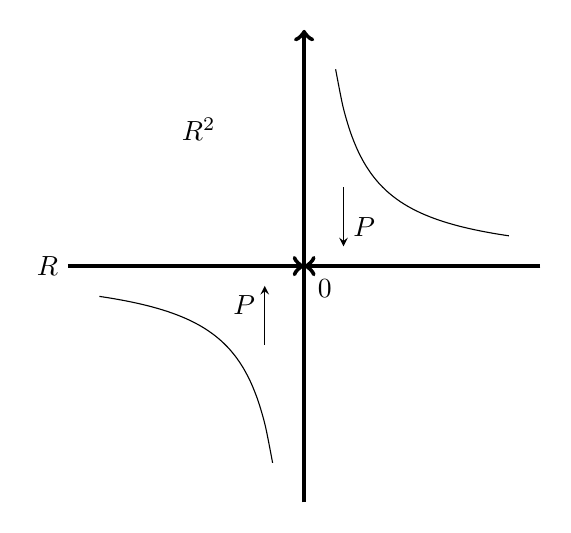
\begin{tikzpicture}
\draw[->, ultra thick] (0,3) -- (3,3);
\draw[->, ultra thick] (6,3) -- (3,3);
\draw[->, ultra thick] (3,0) -- (3,6);

\node[anchor=east] at (0, 3) {$\mathbb{R}$};
\node[anchor=north east] at (2, 5) {$\mathbb{R}^2$};
\node[anchor=north west] at (3.05,2.95) {$0$};

\draw[scale=1, domain=3.4:5.6, smooth, variable=\x, black] plot ({\x}, {1/(\x-3)+3});
\draw[scale=1, domain=0.4:2.6, smooth, variable=\x, black] plot ({\x}, {1/(\x-3)+3});

\draw [-stealth](3.5,4) -- (3.5,3.25) node[anchor=south west] {$P$};
\draw [-stealth](2.5,2) -- (2.5,2.75) node[anchor=north east] {$P$};

\end{tikzpicture}
\end{center}
\end{example}
\par Ինչպես գիտենք, եթե $f:X\rightarrow Y$ և $g:Y\rightarrow Z$ արտապատկերումներն անընդհատ են, ապա նրանց $g\circ f:Y\rightarrow Z$ համադրույթը անընդհատ է։ Քննարկենք հակառակ խնդիրը․ դիցուք հայտնի է, որ $g\circ f$ համադրույթը անընդհատ է, և անընդհատ է $f, g$ արտապատկերումներից մեկը։ Կլինի՞ անընդհատ մյուսը։ Հետևյալ օրինակները ցույց են տալիս, որ ընդհանուր դեպքում հարցի պատասխանը բացասական է։
\begin{example} Դիտարկենք որևէ $f:X\rightarrow Y$ ոչ անընդհատ արտապատկերում և ${g:Y\rightarrow \R},\ g(y)=0,\ y\in\R$ հաստատուն արտապատկերումը։ Պարզ է, որ ${g\circ f:X\rightarrow\R}$ համադրույթը նույնպես հաստատուն արտապատկերում է, և հետևաբար այն անընդհատ է։ Այսպիսով՝ $g\circ f$ –ը և $g$-ն անընդհատ են, բայց $f$-ը անընդհատ չէ։
\end{example}
\par Ընթերցողին առաջարկում ենք բերել նման օրինակ, երբ անընդհատ են $f:X\rightarrow Y$ և $f\circ g:X\rightarrow Z$ արտապատկերումները, բայց անընդհատ չէ $g:Y\rightarrow Z$ արտապատկերումը։
\par Հետևյալ երկու հատուկ դեպքերում $f, g$ արտապատկերումներից մեկի և նրանց $g\circ f$ համադրույթի անընդհատությունից հետևում է նաև մյուսի անընդհատությունը։
\begin{theorem}Ունենք $f:X\rightarrow Y,\ g:Y\rightarrow Z$ արտապատկերումներ, ընդ որում $g\circ f$-ը անընդհատ է․
\begin{enumerate}
    \item [ա)] եթե $g$-ն ինյեկտիվ բաց (կամ փակ) արտապատկերում է, ապա $f$-ը անընդհատ է,
    \item [բ)] եթե $f$-ը սյուրյեկտիվ բաց (կամ փակ) արտապատկերում է, ապա $g$-ն անընդհատ է։
\end{enumerate}
\end{theorem}
\par Ապացուցենք ա)-ն։ Դիցուք $V\subset Y$ ենթաբազմությունը բաց է $Y$-ում, ցույց տանք, որ $f^{-1}(V)$-ն բաց է $X$-ում։ Ըստ պայմանի $g(V)$-ն բաց է $Z$-ում։ Հետևաբար $(g\circ f)^{-1}(g(V))$-ն բաց է $X$-ում։ Ունենք՝ $(g\circ f)^{-1}(g(V))=f^{-1}(g^{-1}\big(g(V)\big)=f^{-1} (V)\Rightarrow f^{-1} (V)$-ն բաց է $X\textrm{-ում} \Rightarrow f$-ը անընդհատ է։ \qed
\par Նման ձևով ապացուցվում է բ)-ն՝ թողնելով այն ընթերցողին։ 
\par Բերենք նաև հոմեոմորֆիզմի հայտանիշ բաց (փակ) արտապատկերումների տերմիններով։
\begin{theorem} Որևէ $f:X\rightarrow Y$ արտապատկերում հոմեոմորֆիզմ է այն և միայն այն դեպքում, երբ $f$-ը բաց (կամ փակ) բիյեկտիվ արտապատկերում է։
\end{theorem}
\begin{proof} Դիցուք $f$-ը հոմեոմորֆիզմ է։ Նշանակում է $f$-ը անընդհատ է, փոխմիարժեք է և նրա $g:Y\rightarrow X$ հակադարձ արտապատկերումը նույնպես անընդհատ է։ Եթե այժմ $U$-ն որևէ բաց ենթաբազմություն է $X$-ում, ապա $f$-ի բիյեկտիվությունից և $g$-ի անընդհատությունից հետևում է, որ $f(U)=g^{-1}(U)$ ենթաբազմությունը բաց է $Y\textrm{-ում}$, ուստի $f$-ը բաց արտապատկերում է։ 
\par Այժմ հակառակը․ դիցուք $f$-ը բաց, բիյեկտիվ արտապատկերում է։ Նշանակում է $f$-ը անընդհատ է և գոյություն ունի նրա հակադարձ $g:Y\rightarrow X$ արտապատկերում։ Մնում է ցույց տալ, որ $g$ արտապատկերումը անընդհատ է։ Եթե $U$-ն որևէ բաց են\-թա\-բազ\-մություն է $X$-ում, ապա $g^{-1}(U)=f(U)$ ենթաբազմությունը բաց է $Y$-ում ըստ պայմանի։
Ուստի $g$-ն անընդհատ է ըստ թեմա 10-ում \hyperlink{sec:10}{թեորեմ $3$}-ի։
\end{proof}
\end{document}